
%(BEGIN_QUESTION)
% Copyright 2006, Tony R. Kuphaldt, released under the Creative Commons Attribution License (v 1.0)
% This means you may do almost anything with this work of mine, so long as you give me proper credit

In the following liquid/vapor filled system (Class II), where is the liquid located in the system, and where is the vapor located in the system?

$$\includegraphics[width=15.5cm]{i00361x01.eps}$$

What will happen to the liquid and vapor locations if the process temperature decreases to 60$^{o}$ F?

\underbar{file i00361}
%(END_QUESTION)





%(BEGIN_ANSWER)

In the illustrated scenario, the liquid will move to the colder location (the indicator mechanism), while the vapor will move to the hotter location (the sensing bulb).  This is typical for Class II filled systems: the liquid portion of the fill will try to migrate to the colder end, while the vapor portion will try to migrate to the warmer end.  Only the Class IID type of system eliminates this problem, by using a non-volatile fill liquid to constantly occupy the capillary tube and sensing element (bourdon tube or bellows), thus confining the volatile liquid and vapor to the bulb.

\vskip 10pt

As the process temperature cools below the indicator element's ambient temperature of 72$^{o}$ F, the liquid will try to migrate to the bulb and the vapor to the indicator.  As this transfer is taking place, the pressure in the system will become unstable, creating unpredictable changes in temperature measurement at the indicator.  This is commonly known as the {\it cross-ambient} problem.

For this reason, Class II filled systems should be avoided when measuring process temperatures ranging above and below ambient (indicator) temperature.

%(END_ANSWER)





%(BEGIN_NOTES)


%INDEX% Measurement, temperature: filled-bulb system

%(END_NOTES)


